\documentclass[a4paper,11pt,twocolumn]{article}

\usepackage{aas_macros}

\usepackage[utf8]{inputenc}
\usepackage[T1]{fontenc}
\usepackage{lmodern}
%\usepackage{times}
%\usepackage[margin=2cm]{geometry}
\usepackage[a4paper]{geometry}
\usepackage{amsmath}
\usepackage{mathtools}
\usepackage{graphicx}
\usepackage{multirow}
\usepackage{multicol}
\usepackage{blindtext}
\usepackage{hyperref}
\usepackage{float}

\usepackage{pgfplotstable}
\usepackage{booktabs}
\pgfplotsset{compat=1.18}

\usepackage[authoryear]{natbib}

\graphicspath{ {./images/} }

\usepackage[czech]{babel}
\usepackage{graphicx}
\usepackage{amsmath}
\usepackage{xspace}
\usepackage{url}
\usepackage{siunitx}
\usepackage{indentfirst}
\usepackage{subcaption}
\usepackage{caption}
\usepackage{tabularx}
\usepackage{rotating}
\usepackage{tikz}
\usepackage[labelformat=parens,labelsep=quad,skip=3pt]{caption}

\usepackage{color}
\usepackage{listings}

\definecolor{codegreen}{rgb}{0,0.6,0}
\definecolor{codegray}{rgb}{0.5,0.5,0.5}
\definecolor{codepurple}{rgb}{0.58,0,0.82}
\definecolor{backcolour}{rgb}{0.95,0.95,0.92}

\lstdefinestyle{mystyle}{
    backgroundcolor=\color{backcolour},
    commentstyle=\color{codegreen},
    keywordstyle=\color{magenta},
    numberstyle=\tiny\color{codegray},
    stringstyle=\color{codepurple},
    basicstyle=\ttfamily\footnotesize\centering,
    breaklines=true,
    captionpos=b,
    numbers=left,
    numbersep=5pt,
    showspaces=false,
    showstringspaces=false,
    showtabs=false,
    tabsize=2
}

\lstset{style=mystyle}

%\widowpenalty 10000 \clubpenalty 10000 \displaywidowpenalty 10000
\setcounter{topnumber}{3}
\setcounter{bottomnumber}{3}
\setcounter{totalnumber}{6}
\renewcommand\topfraction{0.9}
\renewcommand\bottomfraction{0.9}
\renewcommand\textfraction{0.1}
\intextsep=8mm \textfloatsep=8mm

\renewcommand{\thesection}{\arabic{section}.}
\renewcommand{\thesubsection}{\thesection\arabic{subsection}.}
\makeatletter \def\@seccntformat#1{\csname the#1\endcsname\hspace{1ex}} \makeatother

\begin{document}
    \twocolumn[
    \noindent\hrulefill
    \begin{center}
        \bigskip
        \huge ROYGBIV\footnote{\href{https://youtu.be/Scpdj90Z5Nw?si=RcKdZYwc_lgMjFL_}{Public Service Broadcasting - ROYGBIV}}
        \par \large F4191: Praktikum z astronomie 2
        \par \large Artem Gorodilov
        \vspace{0.2cm}
        \par \large 13. ~února 2025
        \bigskip
    \end{center}
    \noindent\hrulefill
    \bigskip
    ]

    \vskip10pt
    \section{Abstrakt}
        V této práci jsem zkombinoval metody ze svých dvou předchozích prací: Určení svítivosti OJ 287 a Pink Floyd, pro vytvoření barevných snímků objektů: M51, M57, M97 a M104.
        
        Výpočty byly provedeny pomocí skriptu v Pythonu \cite{github}.
    \section{Fyzika záření}
        \subsection{M104 (Sombrero Galaxy)}
            \begin{figure}
                \centering
                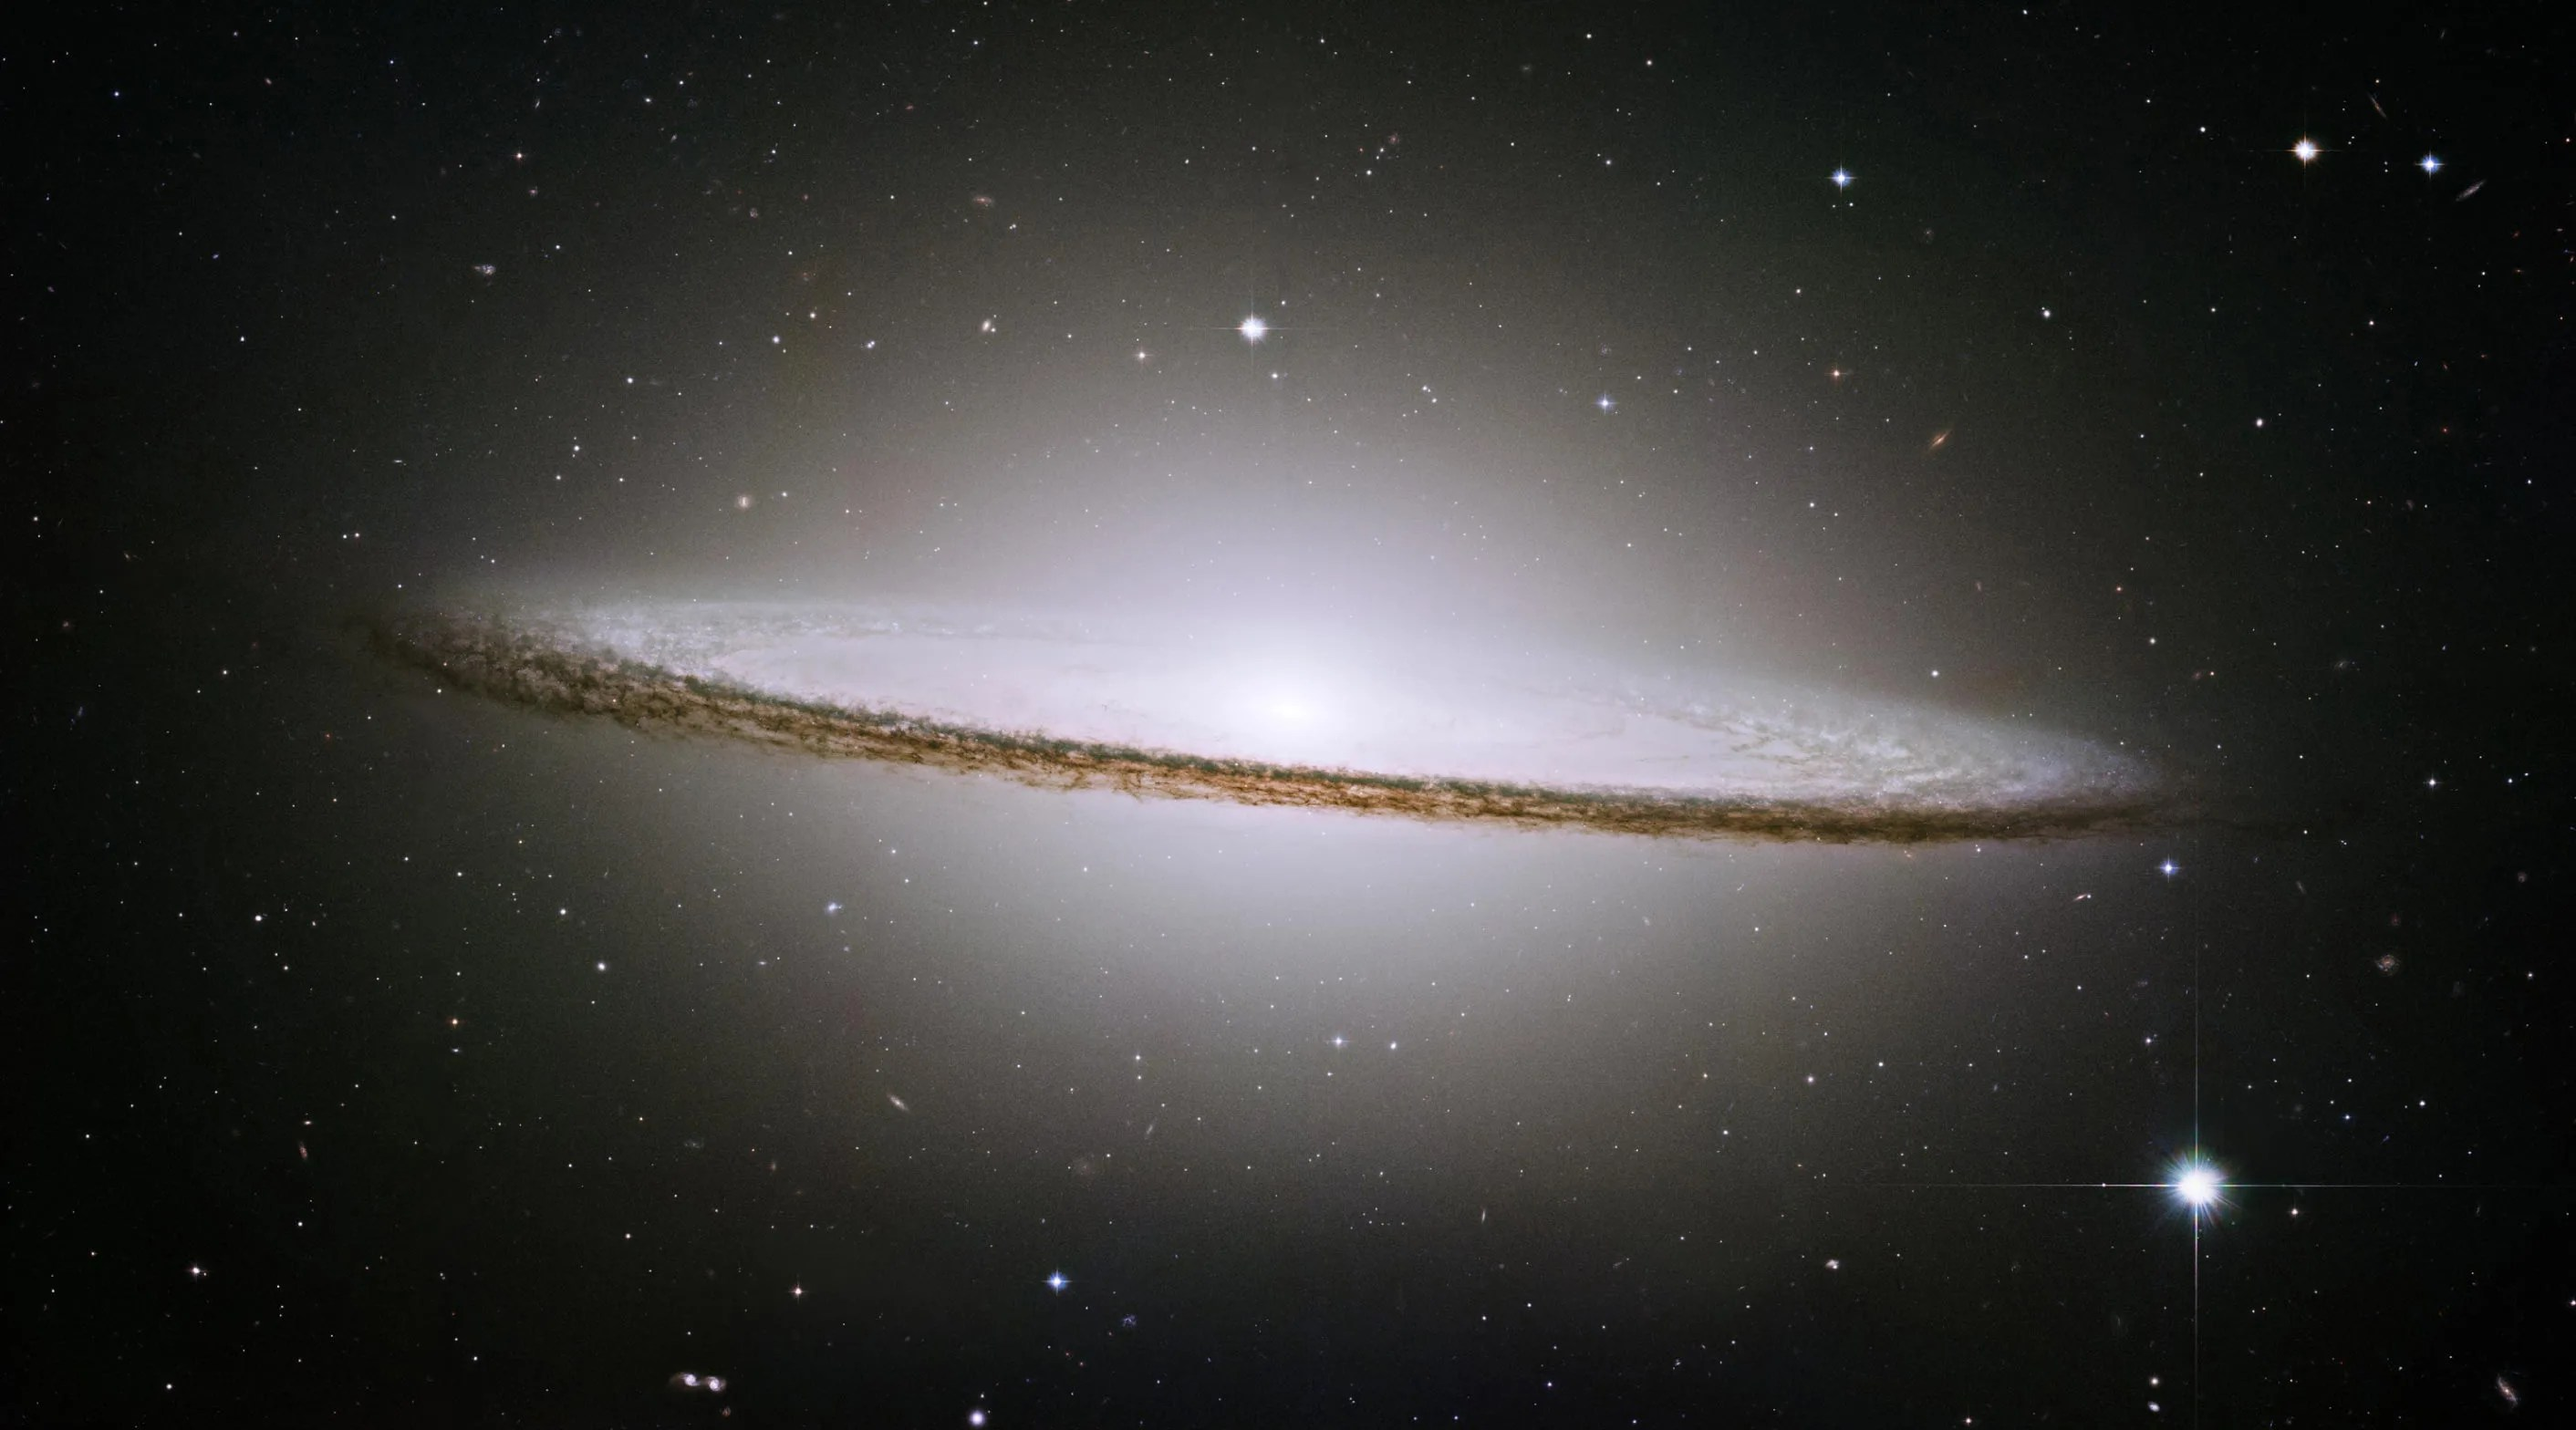
\includegraphics[width=0.5\textwidth]{sombrero.png}
                \caption{Sombrero Galaxy (M104). Source: \href{https://science.nasa.gov/mission/hubble/science/explore-the-night-sky/hubble-messier-catalog/messier-104/}{Messier 104}}
                \label{fig:sombrero}
            \end{figure}

            Galaxie M104 (Sombrero) vykazuje v optickém spektru emisní čáry charakteristické pro nízkoionizované atomy, což naznačuje přítomnost nízkoionizující oblasti v jejím jádru (LINER). Tento typ spektra je často spojován s aktivitou slabých aktivních galaktických jader (AGN) nebo s procesy spojenými se vznikem hvězd.

            Analýza dat z přístroje MUSE na dalekohledu VLT odhalila přítomnost molekulárního prstence v M104, který je detekován prostřednictvím emisí čar $\text{H} \alpha$ a [CII] \citet{sutter2022}. Tyto emise jsou distribuovány v uzlech podél prstence, což naznačuje omezenou aktivní tvorbu hvězd v této oblasti. Poměr [CII]/FIR v M104 je výrazně nižší než u typických hvězdotvorných galaxií a spíše odpovídá hodnotám pozorovaným u raných typů galaxií. To naznačuje, že většina emisí [CII] pochází z ionizovaného a neutrálního atomárního plynu spíše než z molekulárního plynu. 
            
            V blízkosti jádra galaxie byla identifikována prachová struktura interpretovaná jako torus nebo disk, který může kolimovat emise z aktivního galaktického jádra \citet{menezes2013}. Tato struktura je orientována přibližně hranou k pozorovateli, což naznačuje, že pozorované emise mohou být ovlivněny jak kolimací, tak rozptylem světla v okolí jádra. 
            
            Kromě optických emisí M104 vykazuje také emise v infračerveném spektru, které jsou spojeny s přítomností prachových částic v galaxii. Modelování těchto emisí naznačuje, že část prachu je distribuována v klastrech bez přítomnosti embedded zdrojů, což může přispívat k pozorovanému spektru v infračervené oblasti \citet{delooze2012}. 
            
            Celkově lze říci, že emise v galaxii M104 jsou výsledkem kombinace procesů spojených s aktivním galaktickým jádrem, omezenou tvorbou hvězd v molekulárním prstenci a přítomností prachových struktur, které ovlivňují pozorované spektrum v různých vlnových délkách.

        \subsection{M97 (Owl Nebula)}            
            \begin{figure}
                \centering
                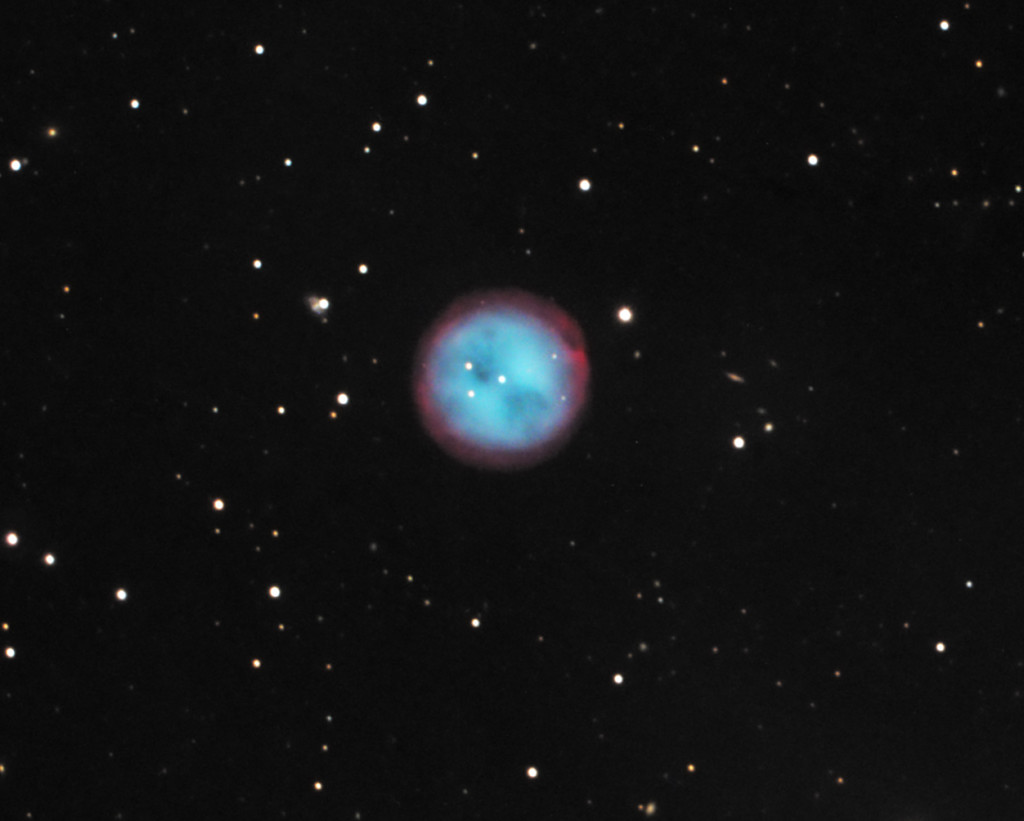
\includegraphics[width=0.5\textwidth]{M97.jpg}
                \caption{Owl Nebula (M97). Source: \href{https://www.messier-objects.com/messier-97-owl-nebula/}{Messier 97: Owl Nebula}}
                \label{fig:m97}
            \end{figure}
            
            Mlhovina M97 (Sova) je planetární mlhovina v souhvězdí Velké medvědice, známá svým charakteristickým kruhovým tvarem a komplexní strukturou. Její optická emise je primárně výsledkem rekombinace ionizovaného vodíku, což vede k výrazné $\text{H} \alpha$ emisní linii. Tento proces nastává, když ultrafialové záření z centrální hvězdy ionizuje okolní plyn; následná rekombinace protonů a elektronů pak vyzařuje fotony v optickém spektru.

            Kromě $\text{H} \alpha$ linie jsou v optickém spektru M97 přítomny i emisní linie dalších prvků, jako je kyslík a dusík. Zejména dvojitě ionizovaný kyslík (O III) produkuje výrazné emisní linie při $4959 \AA$ a $5007 \AA$, které jsou běžné v planetárních mlhovinách a indikují přítomnost oblastí s vyššími teplotami a hustotami \citet{fesen2024}.
            
            V jiných vlnových délkách, jako je infračervené a rádiové spektrum, může M97 vykazovat emise spojené s chladnějším prachem a molekulárním plynem. Studium těchto emisí poskytuje komplexnější pohled na fyzikální podmínky a chemické složení mlhoviny.

        \subsection{M57 (Ring Nebula)}
            \begin{figure}
                \centering
                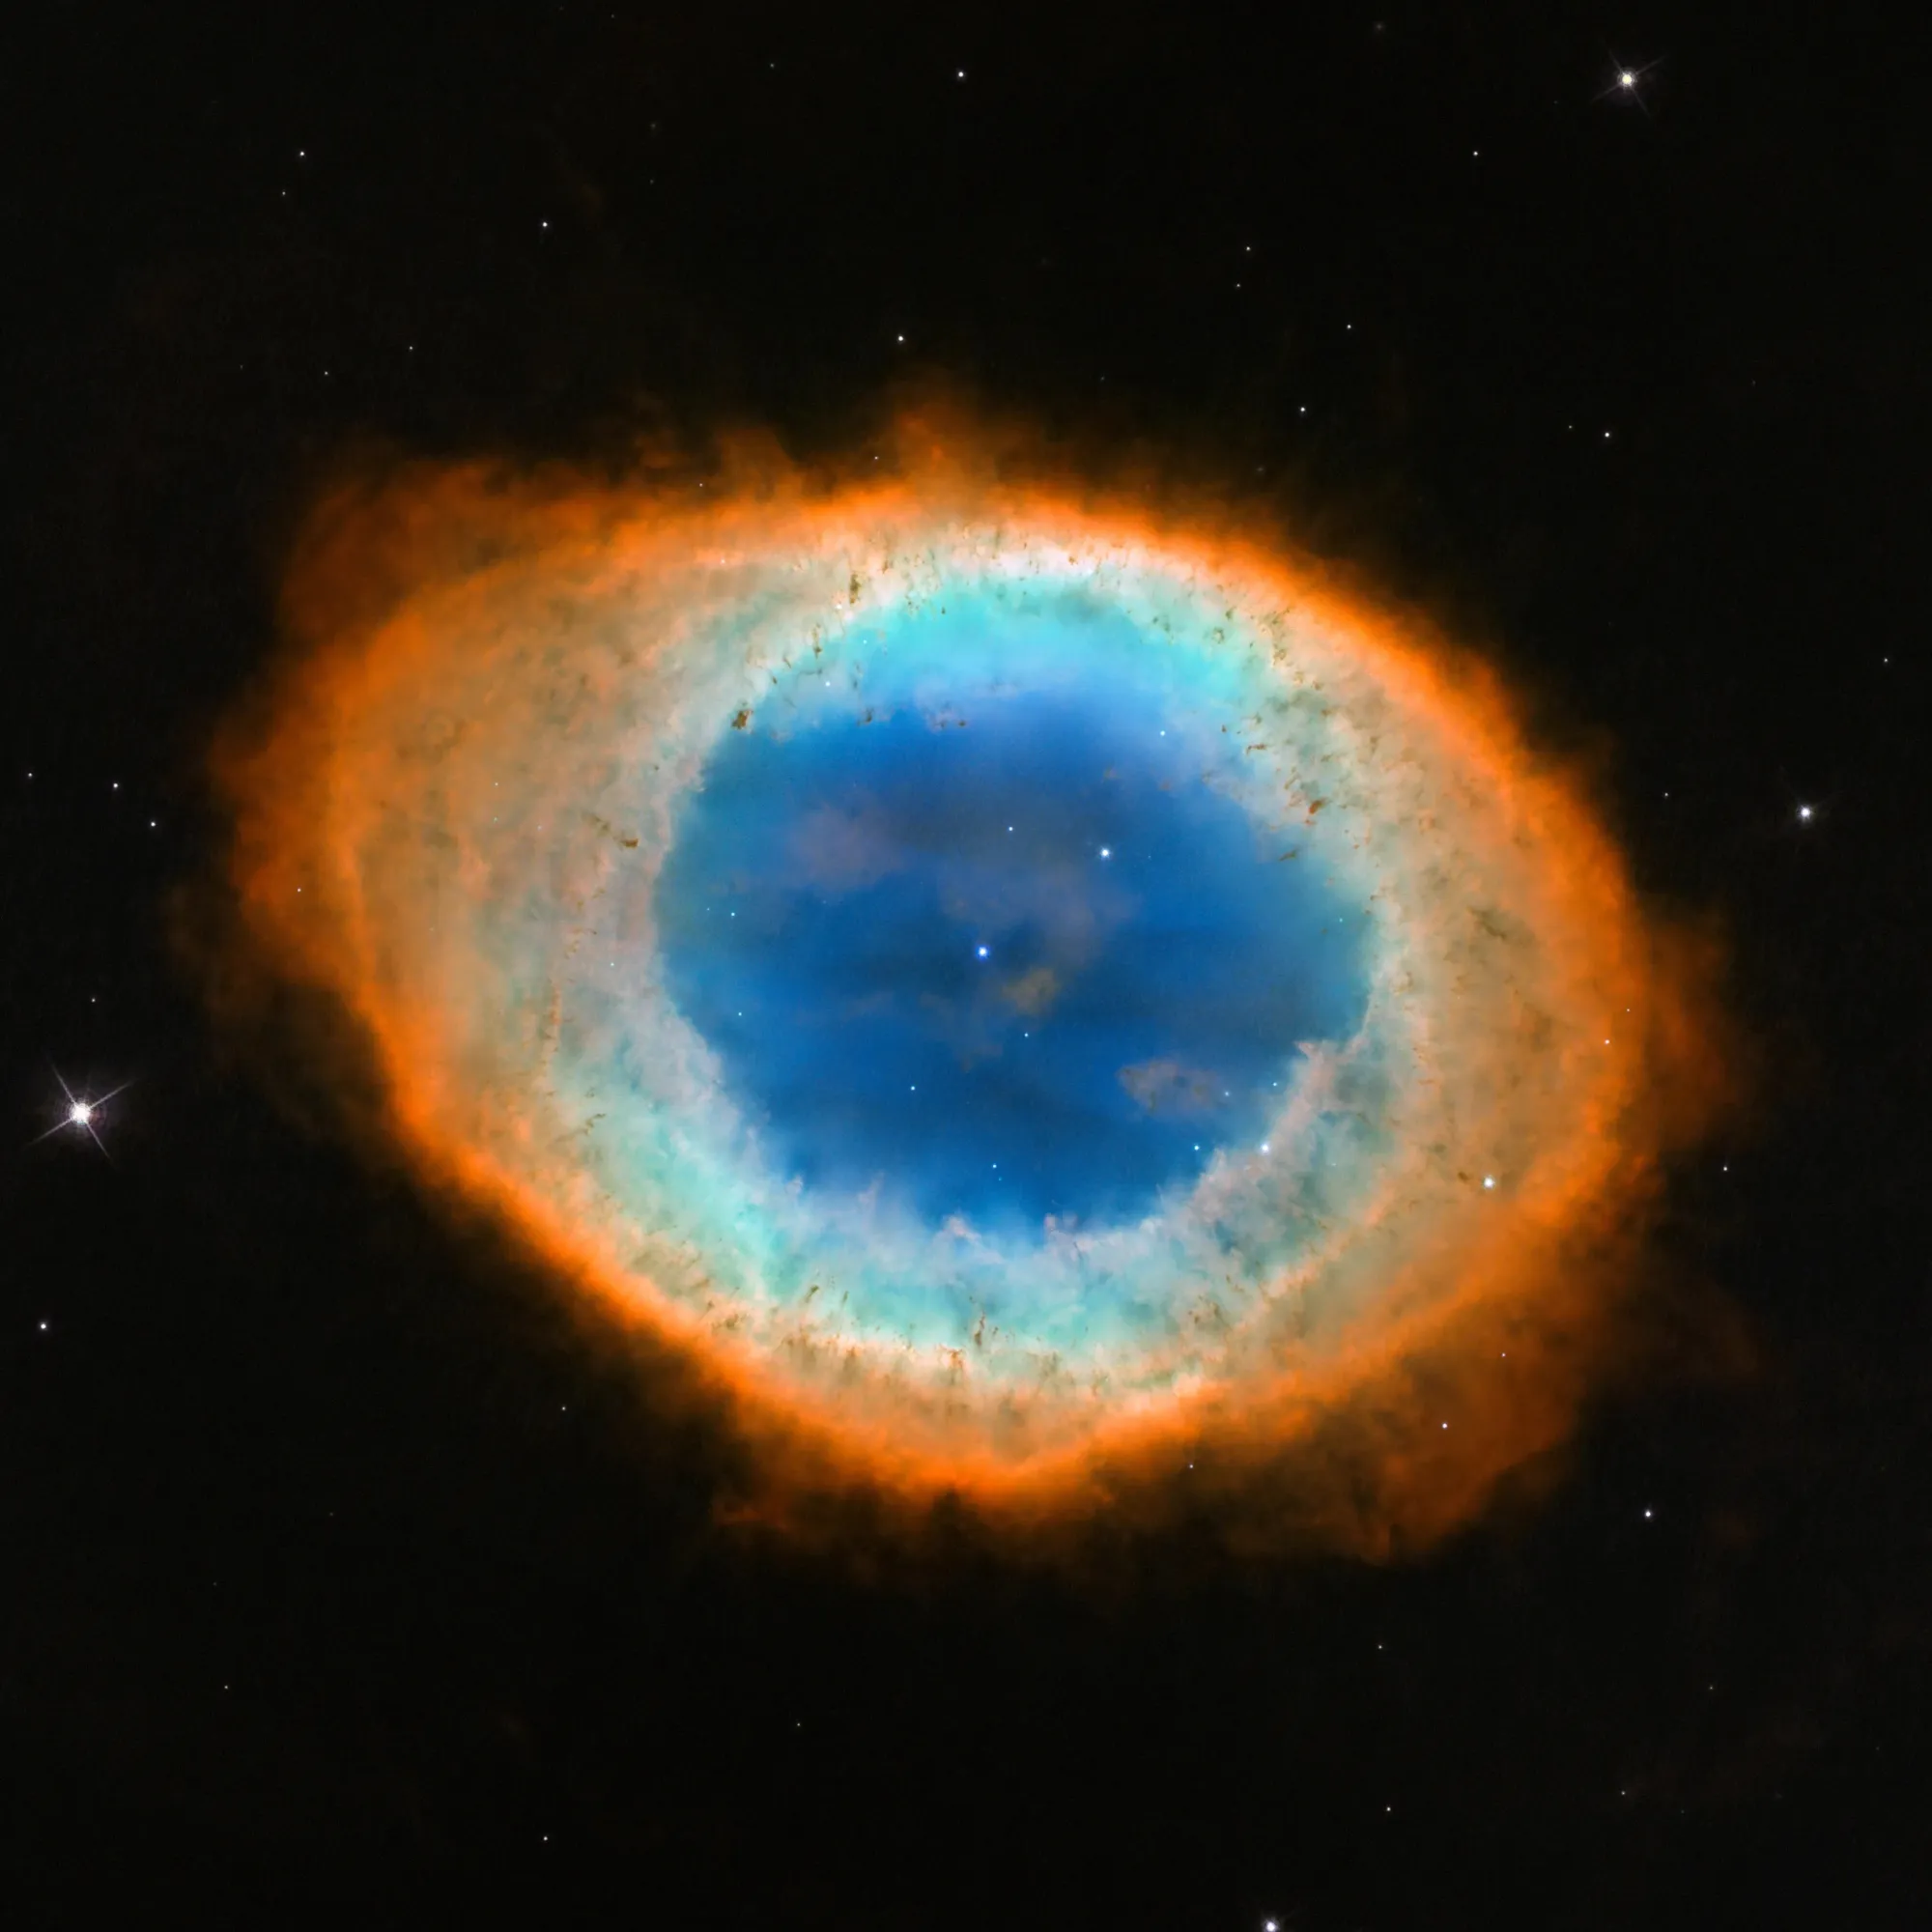
\includegraphics[width=0.5\textwidth]{M57.png}
                \caption{Ring Nebula (M57). Source: \href{https://science.nasa.gov/mission/hubble/science/explore-the-night-sky/hubble-messier-catalog/messier-57/}{Messier 57}}
                \label{fig:m57}
            \end{figure}

            M57 (Prstencová mlhovina) je klasickým příkladem planetární mlhoviny, která vznikla v závěrečných fázích vývoje hvězdy podobné Slunci. Centrální hvězda odvrhla své vnější vrstvy, čímž vytvořila expandující obálku ionizovaného plynu. Optické záření mlhoviny je primárně výsledkem rekombinace a následné emise fotonů z ionizovaných prvků, jako je vodík, helium, kyslík a dusík. Například dvojitě ionizovaný kyslík (O III) emituje charakteristické zelené světlo o vlnové délce $5007 \AA$, což je významný rys ve spektru mnoha planetárních mlhovin \citet{barker1987}.
            
            Kromě optického záření byla v M57 detekována i emise molekulárního vodíku ($\text{H}_\text{2}$) v infračervené oblasti spektra \citet{hoof2010}. Tato emise pochází z fotodissociačních oblastí (PDR), kde ultrafialové záření centrální hvězdy interaguje s neutrálním plynem, což vede k excitaci a následné emisi $\text{H}_\text{2}$. Pozorování pomocí Herschelova vesmírného dalekohledu odhalila, že distribuce prachu v mlhovině úzce souvisí s emisí $\text{H}_\text{2}$, což naznačuje, že molekulární vodík se formuje na povrchu prachových částic. 
            
            Studie středně infračervené spektroskopie pomocí Spitzerova vesmírného dalekohledu identifikovaly v M57 rotační přechody $\text{H}_\text{2}$, což umožnilo odhadnout excitační teplotu molekulárního vodíku kolem $900 \text{K}$ \citet{mata2016}. Tyto výsledky poskytují důležité informace o fyzikálních podmínkách v mlhovině a o procesech formování molekul v pozdních fázích hvězdného vývoje. 

        \subsection{M51 (Whirlpool Galaxy)}
            \begin{figure}
                \centering
                \includegraphics[width=0.5\textwidth]{M51.png}
                \caption{Whirlpool Galaxy (M51). Source: \href{https://science.nasa.gov/missions/hubble/m51-hubble-remix/}{M51 Hubble Remix
                }}
                \label{fig:m51}
            \end{figure}

            V optickém spektru je emise v galaxii M51 (známé též jako Vírová galaxie) dominována zářením mladých, hmotných hvězd, které se nacházejí především ve spirálních ramenech. Tyto oblasti jsou bohaté na mladé hvězdokupy a oblasti ionizovaného vodíku (H II regiony), kde intenzivní ultrafialové záření z nově vzniklých hvězd ionizuje okolní mezihvězdný plyn, což vede k následné rekombinaci a emisi ve viditelném spektru. Studie mladých masivních hvězdokup v M51 ukazují na významnou populaci těchto objektů, které přispívají k celkové optické svítivosti galaxie \citet{larsen2000}.

            V rádiové oblasti spektra je emise M51 charakterizována synchrotronovým zářením, které vzniká při pohybu relativistických elektronů v magnetickém poli galaxie. Polarizované rádiové emise byly detekovány napříč celým diskem M51, přičemž vzor magnetických siločar sleduje optická spirální ramena. Pozorování na frekvencích $1.47 ~ 1.67 \text{GHz}$ odhalila, že distribuce polarizované emise je silně ovlivněna Faradayovou depolarizací, což naznačuje, že polarizovaná emise pochází z horní vrstvy disku, jelikož galaxie není na těchto frekvencích pro polarizovanou emisi transparentní \citet{mulcahy2014}.

            V rentgenovém spektru byla v centrální oblasti M51 detekována emise, která je spojována s aktivním galaktickým jádrem (AGN). Pozorování odhalila bipolární výtoky, které interagují s okolním mezihvězdným médiem a vedou k jeho ohřevu na teploty emitující rentgenové záření \citet{liu2015}. Spektrální analýzy naznačují, že v těchto oblastech může docházet k procesům, jako je rekombinující plazma nebo nárazová excitace, což přispívá k pozorované rentgenové emisi.
        
    \section{Zpracování dat}
        V práci (Určení svítivosti OJ 287) jsem testoval algoritm pro čištění fits snímku s použitím bias, dark a flat snímků (pro BVR filtry). V práci (Pink Floyd) jsem testoval algoritm pro korekci barev a kombinaci několika snímků ve filtrech BVR pro jejich převod na snímky sRGB. Části kódu provádějící tyto funkce byly převzaty z příslušných prací a převedeny na funkce zpracování obrazu pro tuto úlohu. 

        Jediným podstatným rozdílem je přidání metody pro určení bílého bodu. V práci (Pink Floyd) byl zahrnut proces korekce bílého bodu, který vyžadoval nalezení bodu v obraze, který je v případě původního (pravého) obrazu skutečně bílý. V případě plakátu Pink Floyd to byla část světla, která vstupuje do hranolu. V případě obrázků nebeských objektů je situace o něco složitější. Nelze jednoznačně říci, co považovat za bílou barvu, a to ani u původního barevného obrázku. Proto jsem použil následující automatizovaný algoritmus pro určení bodu (hvězdy) s barvou, kterou lze na snímku brát jako bílou. 

        Algoritm funguje takto: 

        \begin{enumerate}
            \item V původních snímcích BVR jsou všechny hvězdy nad určitou úrovní tresholdu nalezeny pomocí funkce \texttt{find\_stars()}.
            \item Hvězdy jsou porovnány podle souřadnic pro každý snímek pomocí funkce \texttt{match\_stars()}, aby bylo zajištěno, že nalezená hvězda je viditelná na všech třech snímcích a nachází se na stejném místě.
            \item Následuje výpočet indexu $B-V$ pro každou hvězdu. To se provede spuštěním funkce \texttt{colour\_images()}. 
            \item Poté je nalezena hvězda s indexem $B-V$ blízkým nule, která odpovídá bílé barvě. 
        \end{enumerate}

        Jde o to, že hvězdy třídy A0V mají $B-V \approx 0$, které lze považovat za bílé. Magnitudy v odpovídajících filtrech se vypočítají jako: 

        \begin{equation}
            m_{\text{filter}} = -2.5 \log_{10} (F_{\text{filter}})
        \end{equation}

        Instrumentální index $(B-V)_{\text{inst}}$ se vypočítá jako:

        \begin{equation}
            (B-V)_{\text{inst}} = m_B - m_V
        \end{equation}

        Pro dosažení lepších výsledků je také nutná korekce Zero-Point:

        \begin{equation}
            (B-V)_{\text{corr}} = (B-V)_{\text{inst}} + ZP
        \end{equation}

        Pro svá data však nemám k dispozici údaje o přesné hodnotě korekce Zero-Point, takže používám pouze index $(B-V)_{\text{inst}}$. 

    \section{Vysledky}
        Pozorování byla provedena v noci z 30.4.2024 na 1.5.2024. Snímky byly získány z \footnote{\url{https://integral.physics.muni.cz/ftp/praktikum/20240430/}}

        Celková doba pozorování jednotlivých objektů byla:

        \begin{equation*}
            \begin{split}
                \text{M104} & : 2490 \text{s} \\
                \text{M97} & : 2010 \text{s} \\
                \text{M57} & : 115 \text{s} \\
                \text{M51} & : 840 \text{s}
            \end{split}
        \end{equation*}

        \subsection{M104 (Sombrero Galaxy)}
            Snímky M104 ve filtrech B, V, R jsou zobrazeny na obrázku (\ref{fig:sombrero_ind.png}). Výsledné BVR, XYZ a sRGB snímky jsou zobrazeny na obrázku (\ref{fig:sombrero_colour.png}).

        \subsection{M97 (Owl Nebula)}
            Snímky M97 ve filtrech B, V, R jsou zobrazeny na obrázku (\ref{fig:M97_ind.png}). Výsledné BVR, XYZ a sRGB snímky jsou zobrazeny na obrázku (\ref{fig:M97_colour.png}).
            
        \subsection{M57 (Ring Nebula)}
            Snímky M57 ve filtrech B, V, R jsou zobrazeny na obrázku (\ref{fig:M57_ind.png}). Výsledné BVR, XYZ a sRGB snímky jsou zobrazeny na obrázku (\ref{fig:M57_colour.png}).
            
        \subsection{M51 (Whirlpool Galaxy)}
            Snímky M51 ve filtrech B, V, R jsou zobrazeny na obrázku (\ref{fig:M51_ind.png}). Výsledné BVR, XYZ a sRGB snímky jsou zobrazeny na obrázku (\ref{fig:M51_colour.png}).

    \section{Závěr}
        Nejlepší barevný snímek byl získán pro galaxii M104 (Sobmrero). Ze snímku je však patrné, že je zřetelně :namodralejší" než původní snímek. U ostatních objektů (M97, M57, M51) je to ještě patrnější. 
            
        Důvodem systematického posunu barevného vyvážení výsledného sRGB snímku do modré oblasti spektra může být použití přístrojového $B-V$ indexu bez Zero Point korekce. V procesu White Spot korekce byla jako referenční bílý bod brána hvězda s $B-V \approx 0$, ale instrumentální hodnoty se mohou lišit od standardních fotometrických hodnot v důsledku kalibračních chyb, vlastností detektoru a atmosféry. Pokud má instrumentální index $B-V$ systematickou odchylku oproti standardním hodnotám, vede to k nesprávné barevné kalibraci, což může vysvětlovat přílišnou modrost výsledného snímku. Kromě toho mohou toto zkreslení zesílit možné rozdíly v citlivosti filtrů a CCD detektoru. Systematický posun barev do modré oblasti tuto hypotézu potvrzuje.

    % \newpage
    \bibliographystyle{abbrvnat}
    \bibliography{bibliography}

    \begin{figure}
        \centering
        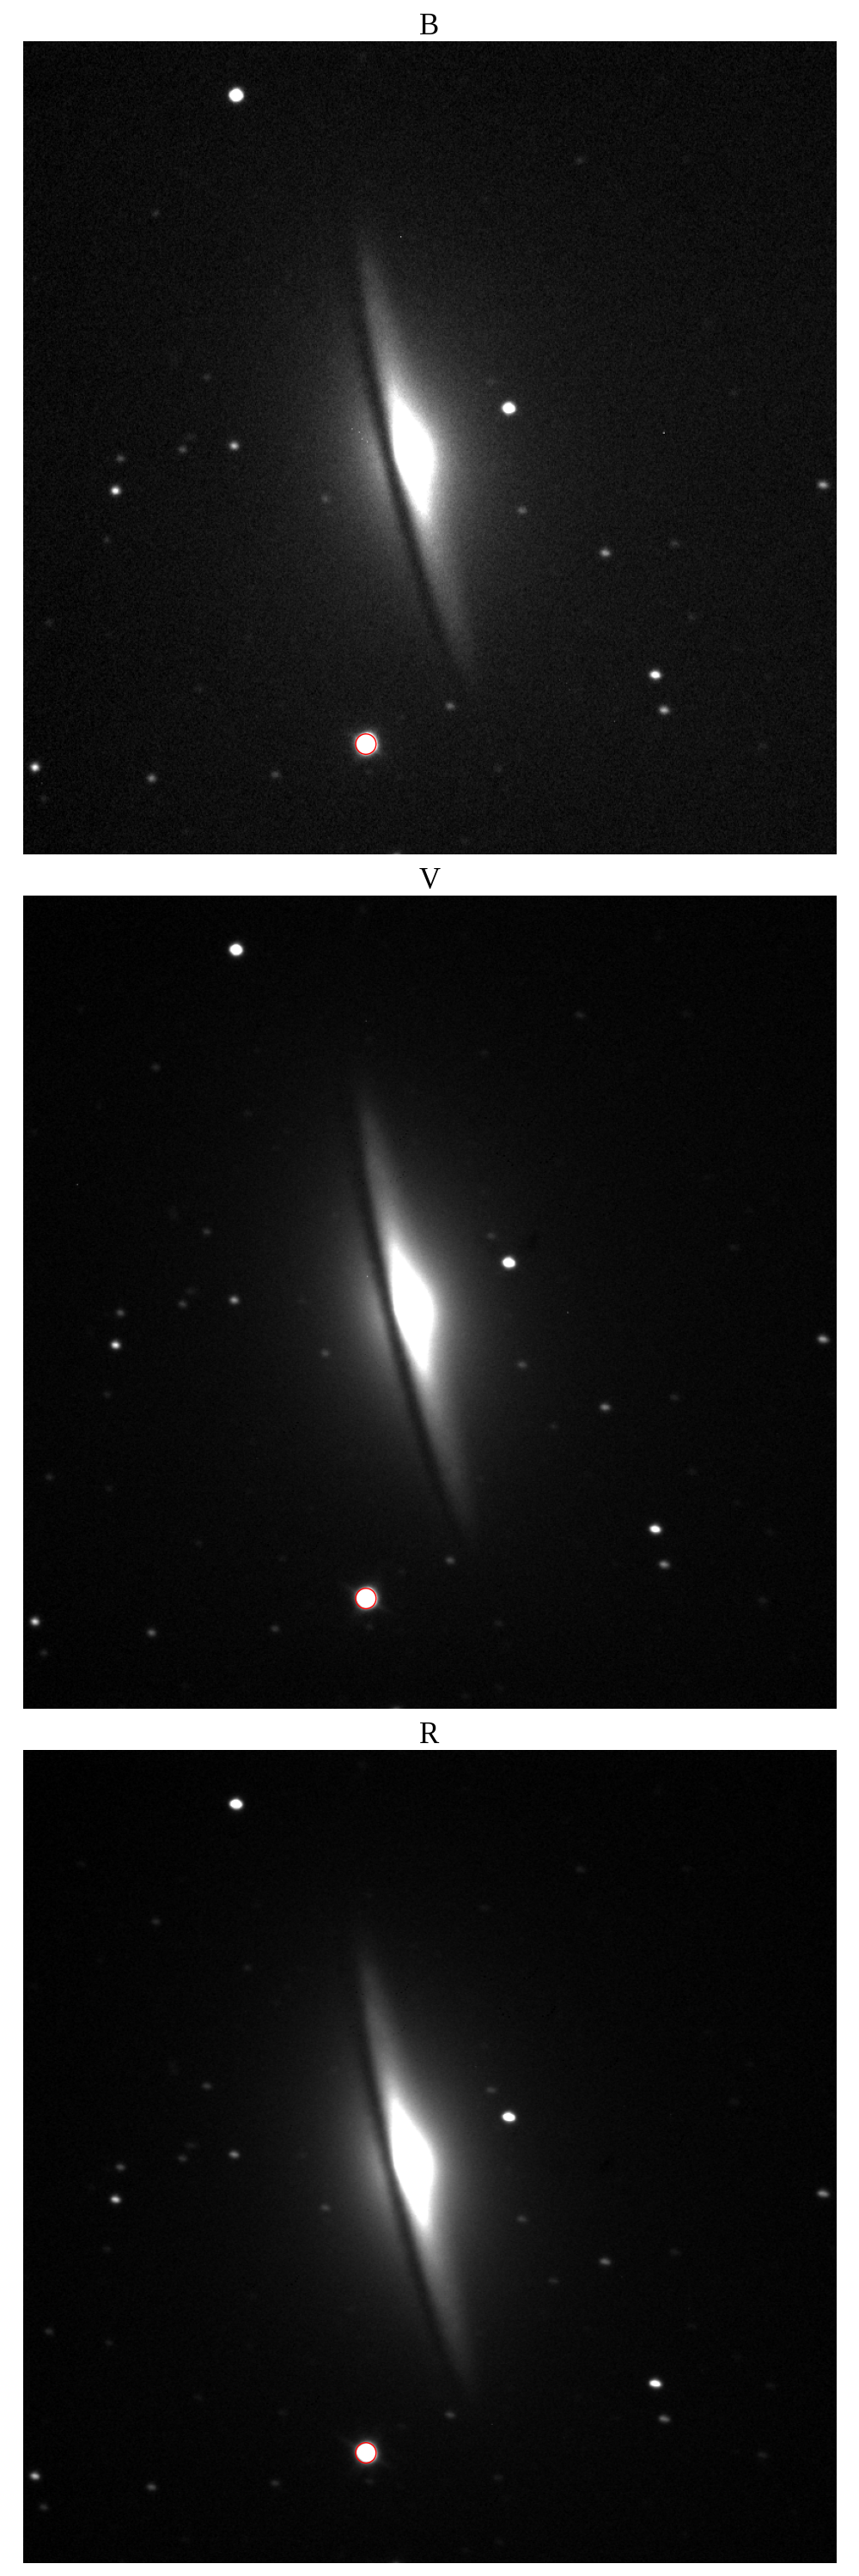
\includegraphics[width=0.5\textwidth]{Sombrero/Sombrero_ind.png}
        \caption{Snímky M104 ve filtrech B, V, R (zhora dolů).}
        \label{fig:sombrero_ind.png}
    \end{figure}

    \begin{figure}
        \centering
        \includegraphics[width=0.5\textwidth]{Sombrero/Sombrero_colour.png}
        \caption{Snímky M104 v barevných systémech BVR, XYZ a sRGB (zhora dolů).}
        \label{fig:sombrero_colour.png}
    \end{figure}

    \begin{figure}
        \centering
        \includegraphics[width=0.5\textwidth]{M97/M97_ind.png}
        \caption{Snímky M97 ve filtrech B, V, R (zhora dolů).}
        \label{fig:M97_ind.png}
    \end{figure}

    \begin{figure}
        \centering
        \includegraphics[width=0.5\textwidth]{M97/M97_colour.png}
        \caption{Snímky M97 v barevných systémech BVR, XYZ a sRGB (zhora dolů).}
        \label{fig:M97_colour.png}
    \end{figure}

    \begin{figure}
        \centering
        \includegraphics[width=0.5\textwidth]{M57/M57_ind.png}
        \caption{Snímky M57 ve filtrech B, V, R (zhora dolů).}
        \label{fig:M57_ind.png}
    \end{figure}

    \begin{figure}
        \centering
        \includegraphics[width=0.5\textwidth]{M57/M57_colour.png}
        \caption{Snímky M57 v barevných systémech BVR, XYZ a sRGB (zhora dolů).}
        \label{fig:M57_colour.png}
    \end{figure}

    \begin{figure}
        \centering
        \includegraphics[width=0.5\textwidth]{M51/M51_ind.png}
        \caption{Snímky M51 ve filtrech B, V, R (zhora dolů).}
        \label{fig:M51_ind.png}
    \end{figure}

    \begin{figure}
        \centering
        \includegraphics[width=0.5\textwidth]{M51/M51_colour.png}
        \caption{Snímky M51 v barevných systémech BVR, XYZ a sRGB (zhora dolů).}
        \label{fig:M51_colour.png}
    \end{figure}

\end{document}